\documentclass[border=3pt]{standalone}
\usepackage{tikz}
\usetikzlibrary{arrows.meta,calc}
\begin{document}
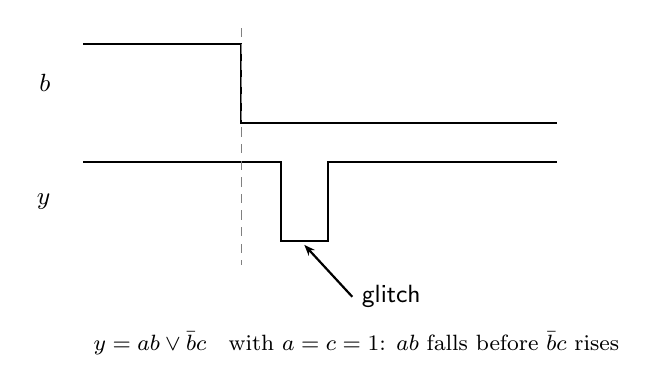
\begin{tikzpicture}[font=\sffamily\small, line cap=rect]
  % b: high then falls at t=2
  \node[left] at (-0.3,0.5) {$b$};
  \draw[thick] (0,1) -- (2,1) -- (2,0) -- (6,0);
  % y = ab + b'c with a=c=1: should stay 1, glitches low
  \node[left] at (-0.3,-1.0) {$y$};
  \draw[thick] (0,-0.5) -- (2.5,-0.5) -- (2.5,-1.5) -- (3.1,-1.5) -- (3.1,-0.5) -- (6,-0.5);
  % transition marker
  \draw[dashed, gray] (2,1.2) -- (2,-1.8);
  % glitch annotation
  \draw[{Stealth[length=4pt]}-, thick] (2.8,-1.55) -- (3.4,-2.2) node[right]{glitch};
  \node[anchor=west, font=\footnotesize] at (0,-2.8) {$y = ab \lor \bar{b}c$ \; with $a = c = 1$: $ab$ falls before $\bar{b}c$ rises};
\end{tikzpicture}
\end{document}
